\documentclass[12pt]{article}
\usepackage{algorithm}
\usepackage{algorithmic}
\usepackage{caption}
\usepackage[a4paper,margin=2.5cm]{geometry}
\usepackage{graphicx}
\usepackage{hyperref}
\usepackage{longtable}
\usepackage{makecell}
\usepackage{multirow}

\title{
	Toward a Systematic Evaluation of Usability in RESTful APIs: A Metric-Based Approach\\
	{\Large \textit{Appendix}}
}

\author{
	Ariel Machini\\
	{\small \texttt{amachini (AT) conicet (DOT) gov (DOT) ar}}
}

\date{March 2026}

\captionsetup{textfont=footnotesize, labelfont=bf, justification=Centering}
\graphicspath{{Figures/}} % Used by graphicx.
\renewcommand{\baselinestretch}{1.25}

\begin{document}
	
	\maketitle
	
	\begin{abstract}
		This document contains complementary content (mostly figures and tables) that could not be included in the main article due to space constraints.
	\end{abstract}
	
	\section{Method}
	
	This Section provides additional information related to the methodological approaches used during the development process of the activities performed.
	
	\subsection{The Goal-Question-Metric approach}
	
	As mentioned in the main article, the Goal-Question-Metric (GQM) approach was leveraged to structurally define the model. For context, a definition of this approach is provided below.
	
	According to \cite{Basili-1994}, ``The result of the application of the Goal Question Metric approach is the specification of a measurement system targeting a particular set of issues and a set of rules for the interpretation of the measurement data''. The resulting measurement model contains three different, but connected levels:
	
	\begin{itemize}
		\item \textbf{Conceptual level (Goals):} Goals are defined for objects, which can be products (artifacts, deliverables, and documents that are produced during the system life cycle), processes (software related activities normally associated with time) and resources (items used by processes in order to produce their outputs).
		\item \textbf{Operational level (Questions):} Questions are used to characterize the way the achievement of a specific goal is going to be performed. Questions try to characterize the object of measurement with respect to a selected quality issue and to determine its quality from the selected viewpoint.
		\item \textbf{Quantitative level (Metrics):} A set of data is associated with every question in order to answer it in a quantitative way. The data can be objective (if they depend only on the object that is being measured) and subjective (if they depend on both the object that is being measured and the viewpoint from which they are taken).
	\end{itemize}
	
	\section{Systematic mapping study}
	
	\subsection{Python scripts}
	While conducting the systematic mapping study, it was found that Springer Link (one of the academic databases used to search for articles) did not allow searching in specific parts of an article, which in turn led to a large number of search results. Additionally, Springer Link only allowed downloading results as a CSV file. To overcome these challenges, two scripts were developed to (1) complete the entries with their corresponding abstracts (whenever possible) and (2) convert the CSV file to a BibTeX file, so it could be fed to JabRef to further narrow the number of results.
	
	\subsubsection{Springer Abstract Scraper}
	The source code for this Python script (which is based on the work of \href{https://github.com/rohitdwivedula}{rohitdwivedula}) is available at \href{https://gist.github.com/arielmachini/f6f299c69230e258f4e49ab9814b3087}{this GitHub gist}.
	
	\subsubsection{Springer2BibTeX}
	The source code for this Python script is available at \href{https://github.com/arielmachini/Springer2BibTeX}{this GitHub repository}.
	
	\subsection{Identified articles}
	In the main article it is mentioned that, as a result of the execution of the systematic mapping study, 18 articles of interest were identified. Table~\ref{tab:SMS-Articles} lists said articles (sorted by year), and Figure~\ref{fig:SMS-Filtering} illustrates the filtering process followed to determine the final set of articles.
	
	\begin{table}
		\centering
		{\footnotesize \begin{tabular}{p{0.5\linewidth}p{0.35\linewidth}p{0.05\linewidth}} % Total width: 0.9\linewidth. 1.0\linewidth exceeds page width.
			\hline
			\textbf{Title} & \textbf{Authors} & \textbf{Year}\\
			\hline
			\textit{Improving Web API Usage Logging} & \cite{SMS-A14} & 2021\\
			\hline
			\textit{Integration of RESTFul API to Student Information System for Secured Data Sharing and Single Sign-on} & \cite{SMS-A3} & 2021\\
			\hline
			\textit{A Data-Driven Approach to Measure the Usability of Web APIs} & \cite{SMS-A4} & 2020\\
			\hline
			\textit{Contexts Enhance Accuracy: On Modeling Context Aware Deep Factorization Machine for Web API QoS Prediction} & \cite{SMS-A2} & 2020\\
			\hline
			\textit{A systematic mapping study of API usability evaluation methods} & \cite{SMS-A9} & 2019\\
			\hline
			\textit{A systematic approach to API usability: Taxonomy-derived criteria and a case study} & \cite{SMS-A8} & 2018\\
			\hline
			\textit{An empirical study for evaluating the performance of multi-cloud APIs} & \cite{SMS-A5} & 2018\\
			\hline
			\textit{Discovering API usability problems at scale} & \cite{SMS-A13} & 2018\\
			\hline
			\textit{QoS-Aware Selection of Web APIs Based on $\varepsilon$-Pareto Genetic Algorithm} & \cite{SMS-A6} & 2016\\
			\hline
			\textit{Automated measurement of API usability: The API Concepts Framework} & \cite{SMS-A11} & 2015\\
			\hline
			\textit{Some structural measures of API usability} & \cite{SMS-A16} & 2015\\
			\hline
			\textit{A quality model for mobile thick client that utilizes web API} & \cite{SMS-A1} & 2014\\
			\hline
			\textit{Towards Understanding of Structural Attributes of Web APIs Using Metrics Based on API Call Responses} & \cite{SMS-A7} & 2014\\
			\hline
			\textit{An Empirical Study of API Usability} & \cite{SMS-A10} & 2013\\
			\hline
			\textit{Methods towards API Usability: A Structural Analysis of Usability Problem Categories} & \cite{SMS-A15} & 2012\\
			\hline
			\textit{The concept maps method as a tool to evaluate the usability of APIs} & \cite{SMS-A17} & 2011\\
			\hline
			\textit{Useful, But Usable? Factors Affecting the Usability of APIs} & \cite{SMS-A18} & 2011\\
			\hline
			\textit{Automatic evaluation of API usability using complexity metrics and visualizations} & \cite{SMS-A12} & 2009\\
			\hline
		\end{tabular}}
		
		\caption{Articles found through the systematic mapping study.}
		\label{tab:SMS-Articles}
	\end{table}
	
	\begin{figure}
		\centering
		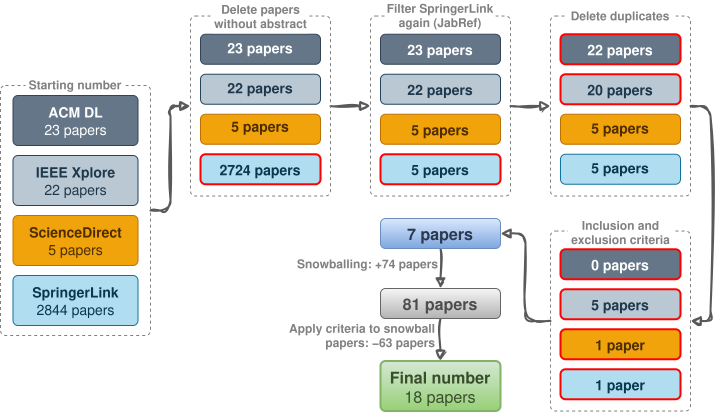
\includegraphics[width=0.7\linewidth]{SMS-Filtering}
		
		\caption{Steps of the filtering process, carried out as part of the systematic mapping study.}
		\label{fig:SMS-Filtering}
	\end{figure}
	
	\section{Goal-Question-Metric usability model}
	As mentioned in the main article, the latest version of the model is composed of six goals (corresponding to the conceptual level), eight questions (operational level), and 45 metrics (quantitative level). Figure~\ref{fig:GQM-Model} presents the different levels and components of the model in a hierarchical manner.
	
	\begin{figure}
		\centering
		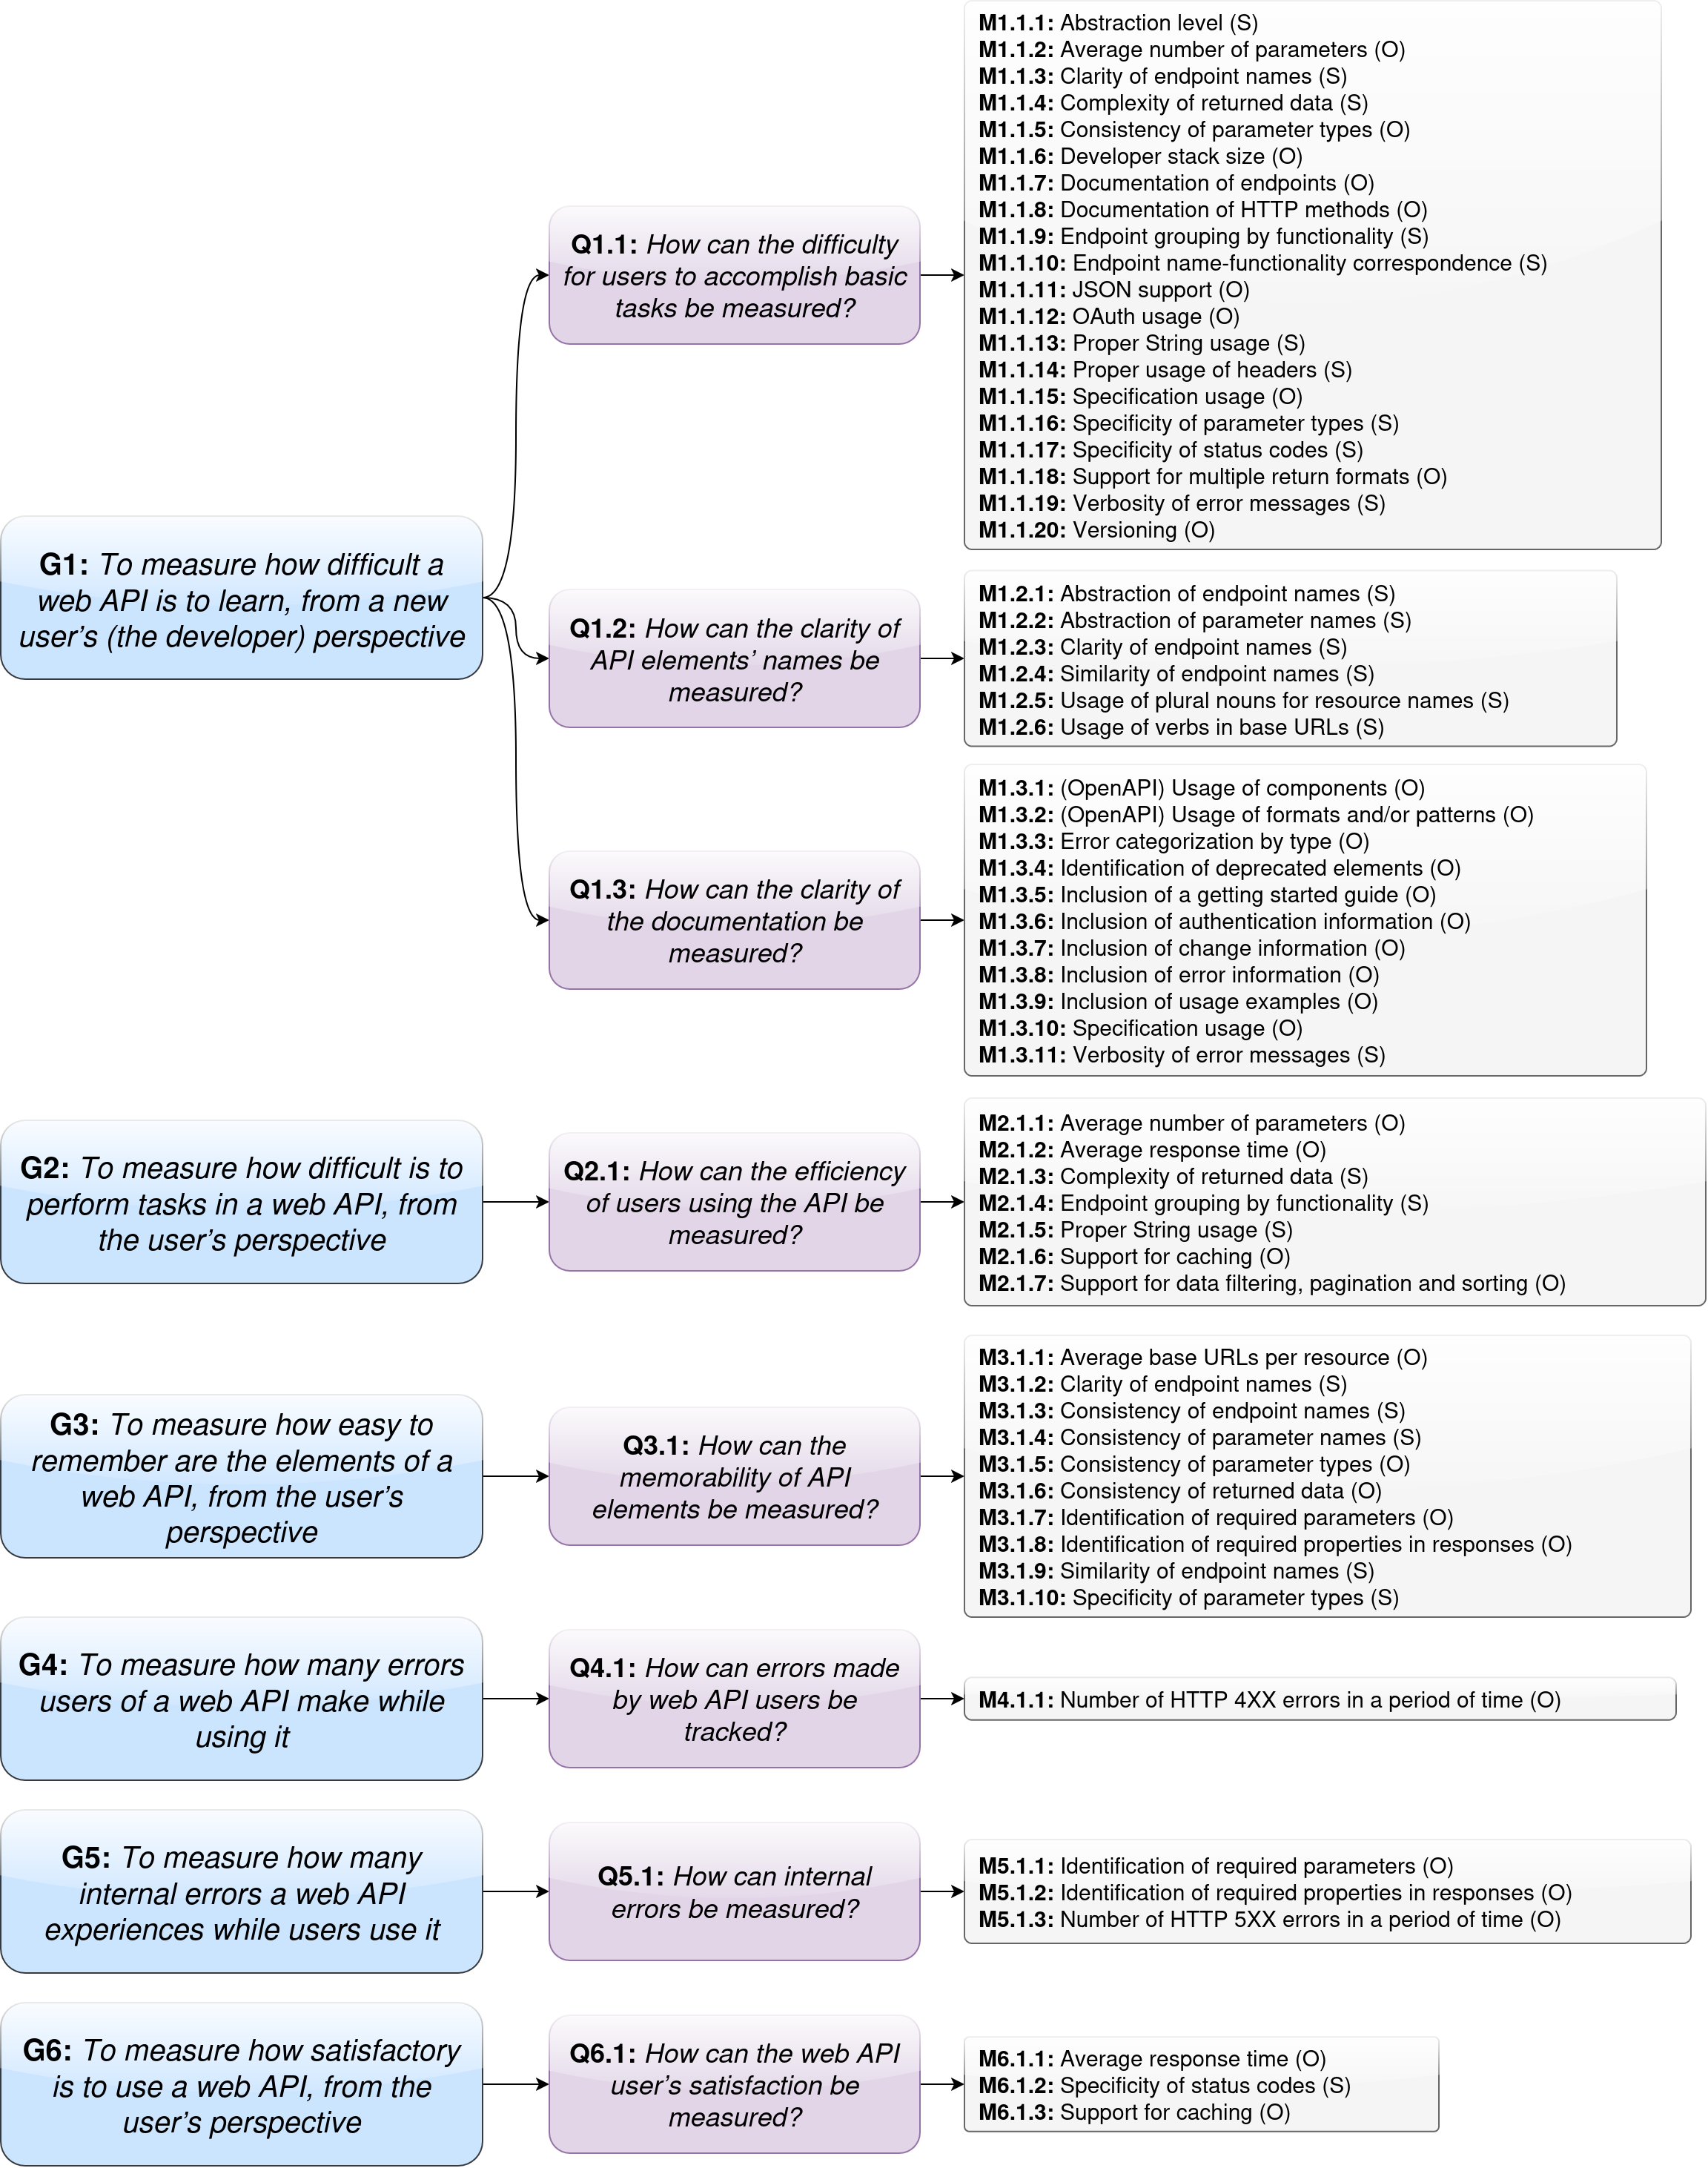
\includegraphics[width=0.9\linewidth]{GQM-Model}
		
		\caption{
			The GQM usability model.\\
			{\scriptsize \textit{Disclaimer:} Please note that the numbering style used to label the metrics is subject to change.}}
		\label{fig:GQM-Model}
	\end{figure}
	
	In the context of the Goal-Question-Metric approach, a metric can be either (O)bjective or (S)ubjective. For context, an objective metric depends only on the object that is being measured, while a subjective metric also depends on the viewpoint from which it is taken \cite{Basili-1994}.
	
	\subsection{Metrics}
	
	Table~\ref{tab:Metrics} details all metrics related to the quantitative level of the proposed model.
	
	\begin{center}
		{\scriptsize \begin{longtable}{p{0.3\linewidth}p{0.6\linewidth}}	
			\hline
			\textbf{Metric} & \textbf{Description}\\
			\hline
			\textbf{Abstraction level} & Abstraction level exposed by the web API. Leaking implementation details can cause confusion for third-party developers and lead to a bad experience.\\
			\hline
			\textbf{Abstraction of endpoint names} & How abstract endpoint names are. Using the right level of abstraction for names helps developers understand what they can do with the web API.\\
			\hline
			\textbf{Abstraction of parameter names} & How abstract parameter names are. Using the right level of abstraction for names helps developers understand what they can do with the web API.\\
			\hline
			\textbf{Average base URLs per resource} & Average number of base URLs per resource. A simple and intuitive base URL design makes a web API easy to use.\\
			\hline
			\textbf{Average number of parameters} & Average number of parameters endpoints have. Long lists of parameters should be avoided when possible.\\
			\hline
			\textbf{Average response time} & Time elapsed from the moment the developer makes a request until it receives a response back. High-performing APIs are considered to have between 0.1 and 1 second average response time. At 2 seconds, the delay is noticeable. At 5 seconds, the delay can cause the developers to abandon the API.\\
			\hline
			\textbf{Clarity of endpoint names} & How clear endpoint names are. Using concise and self-explanatory endpoint names improves the understandability of a web API. Code names, awkward vocabulary, cryptic abbreviations, and having more than three words should be avoided for endpoint names.\\
			\hline
			\textbf{Complexity of returned data} & How complex the data returned by the endpoints that are meant to return something are. Using appropriate data formats for returned data is important to provide a straightforward representation. Avoid overly complex or cryptic data formats. For JSON objects, a maximum depth of 3 and a maximum number of properties of 20 is recommended.\\
			\hline
			\textbf{Consistency of endpoint names} & How consistent endpoint names are. Language and conventions used for naming endpoints should be consistent. A consistent design is easy to understand and use.\\
			\hline
			\textbf{Consistency of parameter names} & How consistent parameter names are. Language and conventions used for naming parameters should be consistent. A consistent design is easy to understand and use.\\
			\hline
			\textbf{Consistency of parameter types} & Whether or not there are parameters with the same name but different types on the web API. Having parameters with identical names but distinct types across different endpoints leads to code bloat in developers' code bases, which negatively impacts usability.\\
			\hline
			\textbf{Consistency of returned data} & How consistent the data returned by the web API are. Language and conventions used for formatting returned data should be consistent. A consistent design is easy to understand and use.\\
			\hline
			\textbf{Developer stack size} & Number of additional tools and libraries a developer has to install in order to use the web API.\\
			\hline
			\textbf{Documentation of endpoints} & Proportion of endpoints that are documented. Ideally, every element of the web API should be documented.\\
			\hline
			\textbf{Documentation of HTTP methods} & Proportion of HTTP methods (part of the endpoints) that are documented. Ideally, every element of the web API should be documented.\\
			\hline
			\textbf{Endpoint grouping by functionality} & Whether or not endpoints with similar functionality are visibly grouped. Grouping endpoints by functionality facilitates navigating through the API and improves understandability. This can be achieved by sorting endpoints in the definition document and leveraging the API specification format.\\
			\hline
			\textbf{Endpoint name-functionality correspondence} & Whether or not the endpoints of the web API perform the tasks suggested by their name. Endpoints should not do less/more than what their names suggest and, if possible, not more than one thing.\\
			\hline
			\textbf{Error categorization by type} & Whether or not errors returned by the web API are grouped or categorized by their meaning. Organizing feedback facilitates interpretation, makes troubleshooting easier and reduces developer frustration.\\
			\hline
			\textbf{Identification of deprecated elements} & Whether or not the documentation of the web API includes deprecated elements. Deprecated elements should be clearly identified.\\
			\hline
			\textbf{Identification of required parameters} & Whether or not all required endpoint parameters are explicitly marked as ``required''. Not doing so might cause unexpected errors and frustration for developers.\\
			\hline
			\textbf{Identification of required properties in responses} & Whether or not all required properties in responses are explicitly marked as ``required''. Not doing so might cause unexpected errors and frustration for developers.\\
			\hline
			\textbf{Inclusion of a getting started guide} & Whether or not the documentation of the web API includes a getting started guide. Having a getting started guide in the documentation helps users to get up and running with the API faster.\\
			\hline
			\textbf{Inclusion of authentication information} & Whether or not the documentation of the web API includes information about authentication (if applicable). Almost every API features some sort of authentication schema, and nearly every one is different. It is because of this that the API documentation should have information on how to access the web API.\\
			\hline
			\textbf{Inclusion of change information} & Whether or not the documentation of the web API includes a changelog section. Having a changelog section in the documentation lets users know how stable the API is. It also lets them know if anything has changed, in case that one of their calls stops working.\\
			\hline
			\textbf{Inclusion of error information} & Whether or not the documentation of the web API includes error information. Ideally, the API documentation should include information about common and important errors.\\
			\hline
			\textbf{Inclusion of usage examples} & Whether or not the documentation of the web API includes usage examples. Ideally, the API documentation should include code samples for the most common scenarios.\\
			\hline
			\textbf{JSON support} & Whether or not the REST API supports the JSON type in requests and/or responses.\\
			\hline
			\textbf{Number of HTTP 4XX errors in a period of time} & Number of client-side errors that occur in a specified period of time. If the number of errors is high with respect to the total number of API calls made in the defined period, documentation might be deficient, naming choices might be poor, or something along these lines may be causing confusion for the web API users.\\
			\hline
			\textbf{Number of HTTP 5XX errors in a period of time} & Number of server-side errors that occurs in a specified period of time. If the number of errors is high with respect to the total number of API calls made in the defined period, the server where the API is hosted might be malfunctioning. This is critical, since it may be motivating enough for developers to look for alternative APIs.\\
			\hline
			\textbf{OAuth usage} & Whether or not the web API supports OAuth for authentication. OAuth is a widely known standard, and using it facilitates user experience.\\
			\hline
			\textbf{Proper String usage} & Whether or not the String type (or an equivalent) is used only when necessary. Strings should not be used if a better type exists, since they are cumbersome and error-prone.\\
			\hline
			\textbf{Proper usage of headers} & Proportion of cases where headers are used appropriately. Defining proper headers helps provide useful information about the server behavior.\\
			\hline
			\textbf{Similarity of endpoint names} & Whether or not there are endpoints with similar names but different functionality. In general, similar names confuse users and increase the chances of making errors.\\
			\hline
			\textbf{Specification usage} & Whether or not the web API provides a specification such as OpenAPI for its users. In addition to serving as a piece of documentation, a specification can help the developer with error checking and validation.\\
			\hline
			\textbf{Usage of components (OpenAPI)} & Whether or not the OpenAPI spec of the web API uses components. Using components makes the OpenAPI specification more readable and removes unnecessary duplication. Components provide a powerful mechanism for defining reusable schemas, parameters, responses, and other elements within the specification.\\
			\hline
			\textbf{Usage of formats and/or patterns (OpenAPI)} & Whether or not the OpenAPI spec of the web API uses formats and/or patterns. Using formats and/or patterns within the OpenAPI spec helps users better understand the kind of values that are expected for a given parameter and add an extra step of validation. Some examples are ``format: uuid'' and ``format: email'' and, if there is no predefined format that suits the data represented by a parameter, the ``pattern'' property can be used to define a regular expression that adapts to it. Note that using formats and/or patterns is not really necessary for simple fields, as this would add unneeded complexity.\\
			\hline
			\textbf{Specificity of parameter types} & Whether or not all types of endpoint parameters are as specific as possible. Data types should be as specific as possible to make the code more readable.\\
			\hline
			\textbf{Specificity of status codes} & How specific status codes returned by the web API are. Ideally, status codes should be as specific as possible, as this could be valuable information for developers and could increase understandability.\\
			\hline
			\textbf{Support for caching} & Whether or not the web API supports caching. In some cases, caching can increase the API performance and, therefore, improve usability. If caching is supported, it should be specified with the Cache-Control header.\\
			\hline
			\textbf{Support for data filtering, pagination and sorting} & Whether or not the web API supports data filtering, pagination and sorting for returned data. Providing developers with these tools improves usability and helps make the web API more adaptable.\\
			\hline
			\textbf{Support for multiple return formats} & Whether or not the web API supports multiple return formats. This helps make the web API more adaptable and improves usability.\\
			\hline
			\textbf{Usage of plural nouns for resource names} & Whether or not resource (endpoint) names are plural when applicable. The use of singular nouns does not give an idea of whether there are multiple items within, leading to confusion, and having both singular and plural nouns will double the API requests list.\\
			\hline
			\textbf{Usage of verbs in base URLs} & Whether or not the web API has endpoints with method-based names. Verbs on endpoint names should be avoided, as they do not convey any new information about the request, since this is handled by the HTTP methods associated with REST.\\
			\hline
			\textbf{Verbosity of error messages} & Verbosity level of error messages returned by the web API. Error feedback must be as informative as possible, so there is no room for confusion.\\
			\hline
			\textbf{Versioning} & Whether or not the web API is versioned. Versioning enables breaking changes to be made with new versions while maintaining backward compatibility for old versions.\\
			\hline
			
			\caption{Final set of metrics related to the quantitative level of the \mbox{Goal-Question-Metric} usability model. These metrics are also used for the catalog.}
			\label{tab:Metrics}
		\end{longtable}}
	\end{center}
	
	\subsection{Automation proof of concept}
	In the main article, more specifically, in Section \textit{Conclusions and future work}, it is pointed out that one of the primary objectives for future work is automating metric assessment (when possible) with a tool that is currently being developed. In this Section, a proof of concept with a single metric (Average base URLs per resource) is provided to exemplify how the automation process will work. Figure~\ref{fig:POC-Flowchart} displays a flowchart summarizing the logic behind the assessment of this particular metric.
	
	\begin{figure}
		\centering
		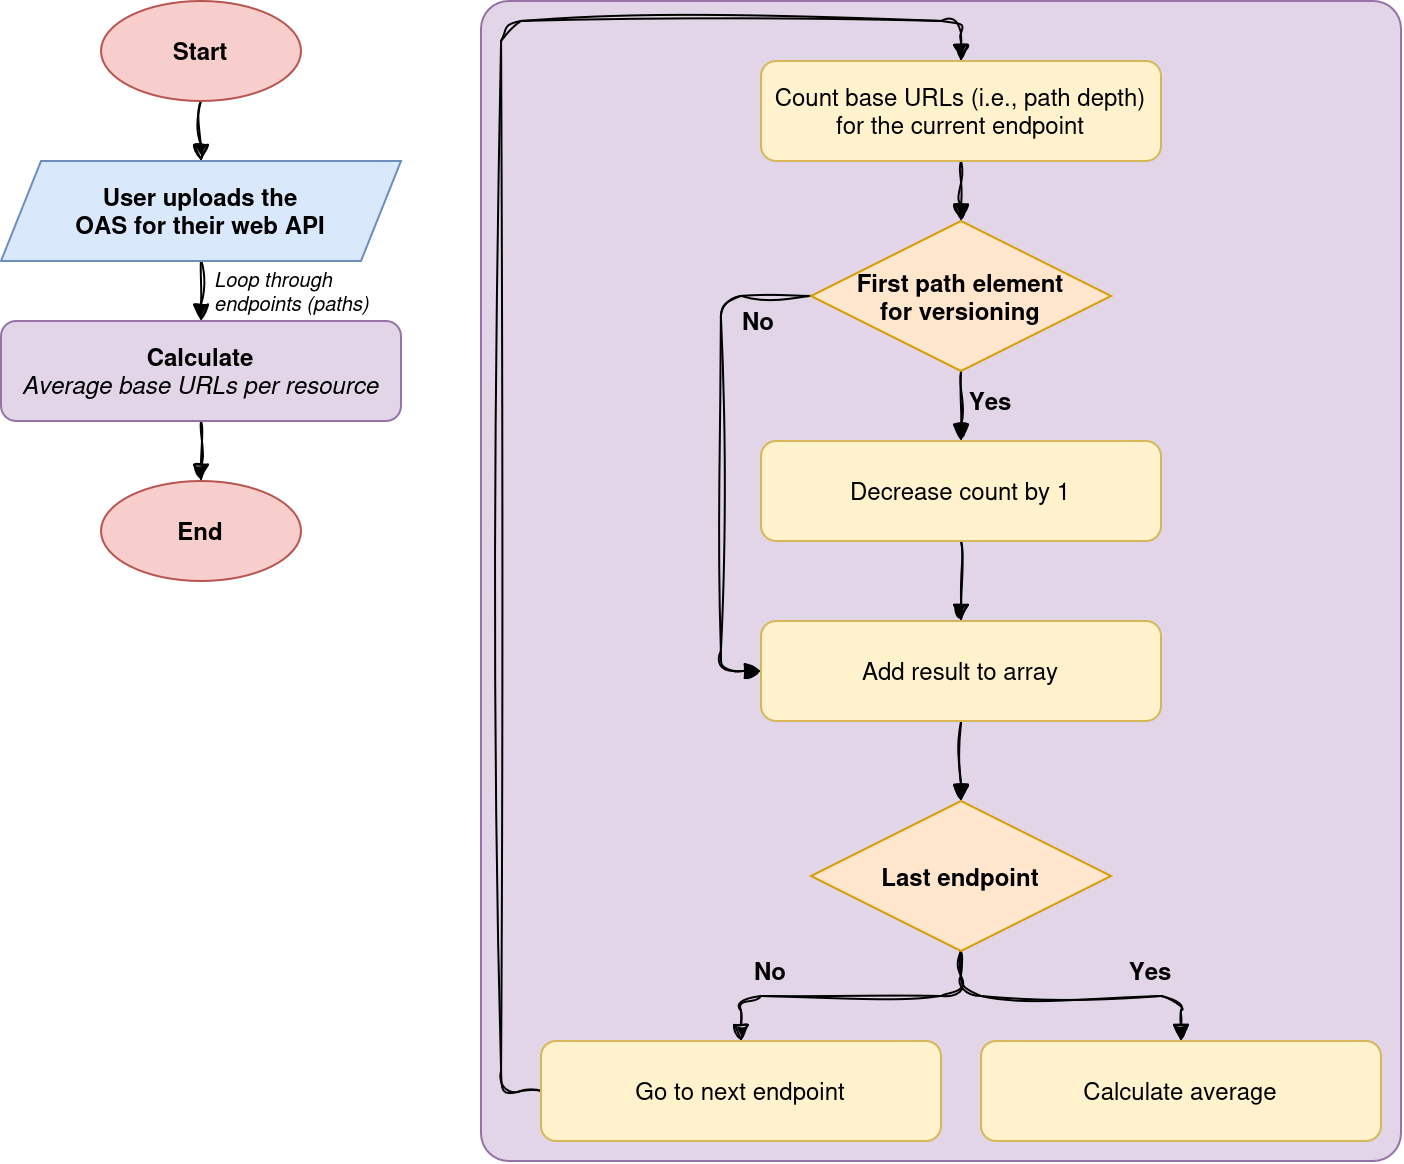
\includegraphics[width=0.8\linewidth]{POC-Flowchart}
		
		\caption{Flowchart for the assessment of ``Average base URLs per resource''.}
		\label{fig:POC-Flowchart}
	\end{figure}
	
	Additionally, Figure~\ref{fig:Proof_of_concept-Pseudocode} presents the pseudocode corresponding to the function that automates the assessment of the aforementioned metric.
	
	\begin{figure}
		{\small \begin{algorithmic}
			\STATE \textbf{function} \texttt{assessAvgBaseURLsPerResource(OAS)} \COMMENT{The OpenAPI spec is user-provided.}
			\STATE \texttt{pathDepthCounts} $\gets$ \texttt{Empty list}
			
			\FORALL{\texttt{path} \textbf{in} \texttt{OAS.paths}}
				\STATE \texttt{explodedPath} $\gets$ List of \texttt{path} components, split by \texttt{/}
				\STATE \texttt{pathDepth} $\gets$ Length of \texttt{explodedPath}
				
				\IF{First element of \texttt{explodedPath} matches versioning pattern (e.g., ``v1'', ``V2.0'')}
					\STATE \texttt{pathDepth} $\gets$ \texttt{pathDepth} - 1
				\ENDIF
				
				\STATE Add \texttt{pathDepth} to \texttt{pathDepthCounts}
			\ENDFOR
			
			\STATE \texttt{avgPathDepth} $\gets$ Sum of \texttt{pathDepthCounts} / Length of \texttt{pathDepthCounts}
			
			\IF{\texttt{avgPathDepth} $\leq$ 2}
				\STATE \texttt{assessmentResult} $\gets$ 1
			\ELSIF{\texttt{avgPathDepth} == 3}
				\STATE \texttt{assessmentResult} $\gets$ 0.5
			\ELSE
				\STATE \texttt{assessmentResult} $\gets$ 0
			\ENDIF
			
			\STATE Update metric ``Average base URLs per resource'' with value \texttt{assessmentResult}
		\end{algorithmic}}
		
		\caption{Pseudocode for the automatic assessment of ``Average base URLs per resource''.}
		\label{fig:Proof_of_concept-Pseudocode}
	\end{figure}
	
	\section{Gwet's AC1 coefficient}
	In the main article, it is stated that ``[s]tatistical analysis of the responses showed substantial agreement''. For clarification, the word \textit{substantial} was taken from \cite{Landis_Koch-1977} and \cite{Wongpakaran-2013}, where the authors indicate that a value above 0.60\footnote{The conducted statistical analysis returned an AC1\cite{Gwet-2008} value of \textbf{0.67}.} indicates \textit{substantial} agreement among the raters.
	
	\clearpage % This prevents figures from interrupting the list of references.
	
	\bibliographystyle{apalike}
	\bibliography{bibliography}
	
\end{document}